\section{Test}
I test sono fondamentali per un'accurata e mirata verifica del prodotto, per questo il gruppo ha deciso di garantire la correttezza continua dell'applicativo parallelizzando i processi di verifica e sviluppo.\\
Nelle sezioni che seguono vengono descritte ed esposte le classi di test che sono state previste per il progetto. Si noti però che al momento nessuna di queste classi esiste in versione \textit{codificata}, ma piuttosto vengono descritte a livello concettuale.

\subsection{Test di unità}
I test di unità sono necessari per controllare le singole unità software presenti nell'applicativo, quali ad esempio classi e metodi, tralasciando quindi le possibili dipendenze con altre componenti.\\
Per questo motivo la dipendenza tra le classi deve essere quanto più sana possibile, ovvero deve esistere solo se effettivamente le due componenti vanno testate insieme.

\subsection{Test d'integrazione}
I test d'integrazione mirano a verificare le comunicazioni e interazioni tra le diverse componenti software. Anche in questo caso, avere dipendenze deboli tra le componenti, permette di superare i test d'integrazione con più facilità.

\subsection{Test di sistema}
I test di sistema sono test che vengono effettuati sulle funzionalità individuate nell'\textit{Analisi dei requisiti}, per verificarne la loro correttezza. \\
Attualmente lo stato di tutti i test riusulta NI ovvero \textit{Non implementato}, l'implementazione sarà oggetto della prossima versione del \textit{Piano di Qualifica}.\\
I codici utilizzati per identificare i test vengono spiegati nel documento \textit{Norme di progetto}, mentre le sigle utilizzate per indicare lo stato del test sono le seguenti: 
\begin{itemize}
    \item \textbf{I}: test implementato
    \item \textbf{NI}: test non implementato
\end{itemize}

%Attenzione! TS2F2 tipo non sono congruenti
\renewcommand{\arraystretch}{1.5}
\begin{longtable}{p{0.12\linewidth}p{0.68\linewidth}p{0.12\linewidth}}
	\rowcolor[RGB]{33, 73, 50}
	\textcolor{white}{\textbf{Codice}} & \textcolor{white}{\textbf{Descrizione}} & \textcolor{white}{\textbf{Stato}}\\
    
    \rowcolor[RGB]{233, 245, 206}
    TS1 & 
    L'utente deve poter caricare i dati nel sistema tramite file \textit{csv}$^{G}$. \par Verificare che: 
    \begin{itemize}
        \item La schermata di caricamento del file sia visualizzata correttamente;
        \item Il formato del file caricato sia corretto;
        \item Il file \textit{csv}$^{G}$ caricato sia ben strutturato;
        \item Il file \textit{csv}$^{G}$ sia sintatticamente corretto;
        \item Venga visualizzato un messaggio d'esito dell'operazione; 
        \item In caso di errore sia possibile ricaricare il file.
    \end{itemize}&
    NI \\

    \rowcolor[RGB]{216, 235, 171}
    TS2 &
    L'utente deve poter scegliere quale tipologia di grafico visualizzare. \par Verificare che:
    \begin{itemize}
        \item Siano presenti dei bottoni per selezionare il grafico da visualizzare;
        \item I bottoni siano parlanti;
        \item Ogni bottone riporti alla visualizzazione del grafico corretta.
    \end{itemize}&
    NI\\

    \rowcolor[RGB]{233, 245, 206}
    TS2.1 & 
    L'utente deve poter visualizzare il grafico \textit{Scatter Plot}$^{G}$. 
    \par Verificare che: 
    \begin{itemize}
        \item L'utente possa associare le dimensioni$^{G}$ agli assi tra quelle disponibili;
        \item Il grafico sia corretto rispetto ai dati da rappresentare;
        \item Il grafico sia coerente con le personalizzazioni adottate \par dall'utente;
        \item L'utente possa interagire con il grafico.
    \end{itemize}&
    NI\\

    \rowcolor[RGB]{216, 235, 171}
    TS2.2 &
    L'utente deve poter visualizzare il grafico \textit{Parallel Coordinates}$^{G}$.
    \par Verificare che:
    \begin{itemize}
        \item L'utente possa associare le dimensioni$^{G}$ agli assi tra quelle disponibili;
        \item Il grafico sia corretto rispetto ai dati da rappresentare;
        \item Il grafico sia coerente con le personalizzazioni adottate \par dall'utente;
        \item L'utente possa interagire con il grafico.
    \end{itemize}&
    NI\\

    \rowcolor[RGB]{233, 245, 206}
    TS2.3 &
    L'utente deve poter visualizzare il grafico \textit{Force-directed Graph}$^{G}$.
    \par Verificare che:
    \begin{itemize}
        \item Ogni variabile abbia il suo corrispettivo nodo nel grafico;
        \item Ogni relazione sia rappresentata da una linea di collegamento tra i
        nodi;        
        \item Il grafico sia corretto rispetto ai dati da rappresentare;
        \item Il grafico sia coerente con le personalizzazioni adottate \par dall'utente;
        \item L'utente possa interagire con il grafico.
    \end{itemize}&
    NI\\

    \rowcolor[RGB]{216, 235, 171}
    TS2.4 &
    L'utente deve poter visualizzare il grafico \textit{Sankey Diagram}$^{G}$.
    \par Verificare che:
    \begin{itemize}
        \item L'utente possa associare le dimensioni$^{G}$ agli assi tra quelle disponibili;
        \item Il grafico sia corretto rispetto ai dati da rappresentare;
        \item Il grafico sia coerente con le personalizzazioni adottate \par dall'utente;
        \item L'utente possa interagire con il grafico.
    \end{itemize}&
    NI\\

    \rowcolor[RGB]{233, 245, 206}
    TS3 & 
    L'utente deve poter tornare alla visualizzazione di default di un grafico. \par 
    Verificare che:
    \begin{itemize}
        \item Sia presente un bottone per tornare alla visualizzazione di default;
        \item Venga visualizzato un messaggio di conferma;
        \item Una volta cliccato il bottone, il grafico sia ritornato alla vista$^{G}$ di default.
    \end{itemize}&
    NI\\

    \rowcolor[RGB]{216, 235, 171}
    TS4 &
    L'utente deve poter personalizzare i grafici, sia visivamente che nel loro contenuto. \par
    Verificare che:
    \begin{itemize}
        \item Sia presente un bottone per personalizzare il grafico;
        \item Il bottone deve essere chiaro e ben visibile;
        \item Una volta cliccato il bottone venga visualizzata la pagina per la personalizzazione.
    \end{itemize}&
    NI\\

    \rowcolor[RGB]{233, 245, 206}
    TS4.1 &
    L'utente deve poter personalizzare il grafico \textit{Scatter Plot}$^{G}$. \par
    Verificare che:
    \begin{itemize}
        \item L'utente possa associare le dimensioni$^{G}$ agli assi tra quelle disponibili;
        \item L'utente possa personalizzare lo stile del grafico;
        \item In caso di errore appaia l'apposito messaggio esplicativo.
    \end{itemize}&
    NI \\

    \rowcolor[RGB]{216, 235, 171}
    TS4.2 &
    L'utente deve poter personalizzare il grafico \textit{Parallel Coordinates}$^{G}$. \par
    Verificare che:
    \begin{itemize}
        \item L'utente possa associare le dimensioni$^{G}$ agli assi tra quelle disponibili;
        \item L'utente possa scegliere l'ordine ed il numero degli assi del grafico;
        \item L'utente possa scegliere lo scaling$^{G}$ dei dati;
        \item L'utente possa personalizzare lo stile del grafico;
        \item In caso di errore appaia l'apposito messaggio esplicativo.
    \end{itemize}&
    NI \\

    \rowcolor[RGB]{233, 245, 206}
    TS4.3 &
    L'utente deve poter personalizzare il grafico \textit{Force-directed Graph}$^{G}$. \par
    Verificare che:
    \begin{itemize}
        \item L'utente possa scegliere l'algoritmo d'integrazione tra quelli disponibili;
        \item L'utente possa scegliere la funzione di forza tra quelle disponibili;
        \item L'utente possa personalizzare lo stile del grafico;
        \item In caso di errore appaia l'apposito messaggio esplicativo.
    \end{itemize}&
    NI \\ 

    \rowcolor[RGB]{216, 235, 171}
    TS4.4 &
    L'utente deve poter personalizzare il grafico \textit{Sankey Diagram}$^{G}$. \par
    Verificare che:
    \begin{itemize}
        \item L'utente possa scegliere l'ordinamento dei dati relativi al grafico;
        \item L'utente possa personalizzare lo stile del grafico;
        \item In caso di errore appaia l'apposito messaggio esplicativo.
    \end{itemize}&
    NI \\

    \rowcolor[RGB]{233, 245, 206}
    TS5 &
    L'utente deve poter visualizzare un grafico a schermo intero. \par 
    Verificare che:
    \begin{itemize}
        \item Sia presente un bottone per la visualizazione a schermo intero;
        \item Una volta cliccato il bottone, il grafico si ridimensioni a schermo intero.
    \end{itemize}&
    NI \\

    \rowcolor[RGB]{216, 235, 171}
    TS6 &
    L'utente deve poter effettuare lo zoom sul grafico. \par 
    Verificare che:
    \begin{itemize}
        \item L'utente sul grafico \textit{Scatter Plot}$^{G}$ possa effettuare lo zoom ad area;
        \item L'utente sul grafico \textit{Force-directed Graph}$^{G}$ possa effettuare lo zoom con lo scroll.
    \end{itemize}&
    NI \\

    \rowcolor[RGB]{233, 245, 206}
    TS7 &
    L'utente deve poter ottenere delle informazioni utili passando con il mouse su alcuni punti del grafico;\par
    Verificare che:
    \begin{itemize}
        \item Le informazioni mostrate una volta eseguito l'hover siano corrette;
        \item Vengano evidenziati gli elementi su cui l'utente esegue la funzionalità di hover.
    \end{itemize}&
    NI \\

    \rowcolor[RGB]{216, 235, 171}
    TS8 &
    L'utente deve poter creare una nuova vista$^{G}$ personalizzata; \par
    Verificare che:
    \begin{itemize}
        \item Sia presente un bottone per la creazione di una nuova vista$^{G}$;
        \item Una volta cliccato il bottone, venga visualizzata la pagina di creazione;
        \item Sia possibile scegliere quali celle/righe/colonne visualizzare;
        \item In caso di errore appaia l’apposito messaggio esplicativo.
    \end{itemize}&
    NI \\

    \rowcolor[RGB]{233, 245, 206}
    TS8.1 &
    L'utente deve poter creare una nuova vista$^{G}$ su \textit{Scatter Plot}$^{G}$. \par
    Verificare che:
    \begin{itemize}
        \item L'utente possa scegliere quali dimensioni$^{G}$ associare agli assi del grafico;
        \item Il grafico venga mostrato secondo le scelte selezionate dall'utente;
        \item In caso di errore appaia l’apposito messaggio esplicativo.
    \end{itemize}&
    NI \\

    \rowcolor[RGB]{216, 235, 171}
    TS8.2 & 
    L'utente deve poter creare una nuova vista$^{G}$ su \textit{Parallel Coordinates}$^{G}$. \par
    Verificare che:
    \begin{itemize}
        \item L'utente possa associare le dimensioni$^{G}$ agli assi tra quelle disponibili;
        \item L'utente possa scegliere l'ordine ed il numero degli assi del grafico;
        \item L'utente possa scegliere lo scaling$^{G}$ dei dati;
        \item In caso di errore appaia l’apposito messaggio esplicativo.
    \end{itemize}&
    NI \\

    \rowcolor[RGB]{233, 245, 206}
    TS8.3 &
    L'utente deve poter creare una nuova vista$^{G}$ su \textit{Force-directed Graph}$^{G}$. \par
    Verificare che:
    \begin{itemize}
        \item L'utente possa scegliere l'algoritmo d'integrazione tra quelli disponibili;
        \item L'utente possa scegliere la funzione di forza tra quelle disponibili;
        \item In caso di errore appaia l’apposito messaggio esplicativo.
    \end{itemize}&
    NI \\

    \rowcolor[RGB]{216, 235, 171}
    TS8.4 &
    L'utente deve poter creare una nuova vista$^{G}$ su \textit{Sankey Diagram}$^{G}$. \par
    Verificare che:
    \begin{itemize}
        \item L'utente possa scegliere l'ordinamento dei dati relativi al grafico;
        \item L'utente possa personalizzare lo stile del grafico;
        \item In caso di errore appaia l'apposito messaggio esplicativo.
    \end{itemize}&
    NI \\

    \rowcolor[RGB]{233, 245, 206}
    TS9 &
    L'utente deve poter salvare le viste$^{G}$ personalizzate. \par
    Verificare che:
    \begin{itemize}
        \item Sia presente un bottone per salvare la vista$^{G}$.
        \item La vista$^{G}$ venga correttamente tradotta in formato \textit{.json}$^{G}$
        \item In caso di errore appaia l'apposito messaggio esplicativo.
    \end{itemize}&
    NI \\

    \rowcolor[RGB]{216, 235, 171}
    TS10 &
    L'utente deve poter caricare una vista$^{G}$ personalizzata nell'applicativo. \par
    Verificare che:
    \begin{itemize}
        \item Sia presente un bottone per caricare la vista$^{G}$.
        \item il file \textit{.json}$^{G}$ relativo alla vista sia ben strutturato;
        \item il file \textit{.json}$^{G}$ relativo alla vista sia sintatticamente corretto;
        \item In caso di errore appaia l'apposito messaggio esplicativo.
    \end{itemize}&
    NI \\

    \rowcolor[RGB]{233, 245, 206}
    TS11 &
    L'utente deve poter eliminare una vista$^{G}$ personalizzata. \par
    Verificare che:
    \begin{itemize}
        \item Sia presente un bottone per eliminare la vista$^{G}$.
        \item Prima dell'eliminazione effettiva appaia l'apposito messaggio di conferma eliminazione.
    \end{itemize}&
    NI \\

    \caption{Tabella dei test di sistema}
\end{longtable}	 

\newpage
\section{Resoconto Test}
\subsection{MPC1 - MPC2}
\begin{figure}[h!]
    \centering
    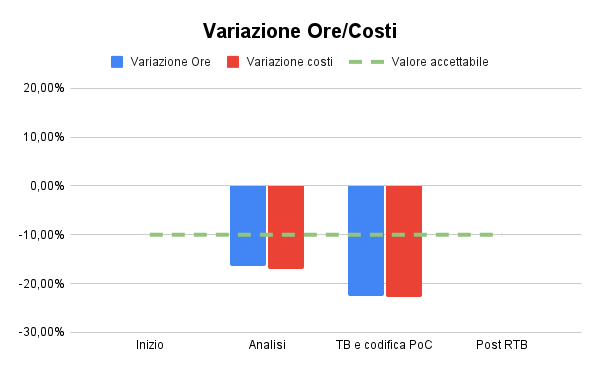
\includegraphics[scale=0.65]{../../assets/Variazione_ore-costi.png}
    \caption{Variazione ore/costi per fase}
\end{figure}

\subsection{MPD1}
\begin{figure}[h!]
    \centering
    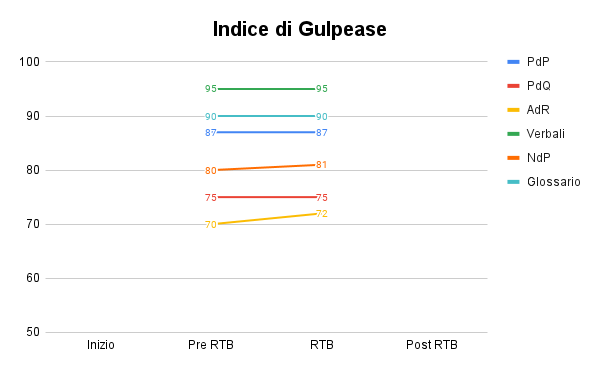
\includegraphics[scale=0.62]{../../assets/Indice di Gulpease.png}
    \caption{Indice di Gulpease}
\end{figure}
\newpage
\subsection{MPD2}
\begin{figure}[h!]
    \centering
    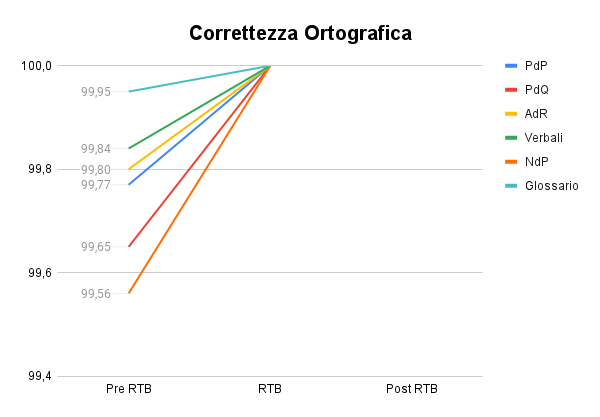
\includegraphics[scale=0.65]{../../assets/correttezza_ortografica.png}
    \caption{Correttezza ortografica dei documenti}
\end{figure}